% !TeX TXS-program:compile = txs:///lualatex

\documentclass[a4paper,11pt]{article}
\usepackage[revgoku]{cp-base}
\graphicspath{{./graphics/}}
%variables.
\donnees[classe={1\up{ère} 2M2},matiere={[SPÉ.MATHS]},mois={Jeudi 16 Décembre},annee=2021,typedoc=TEST~,numdoc=4,duree={15 minutes}]
%formatage
\author{Pierquet}
\title{\nomfichier}
\hypersetup{pdfauthor={Pierquet},pdftitle={\nomfichier},allbordercolors=white,pdfstartview=FitH}
%divers
\lhead{\entete{Durée : \duree}}
\chead{\entete{\lycee}}
\rhead{\entete{\classe{} - \mois{} \annee}}
\lfoot{\pied{\matiere}}
\cfoot{\logolycee{}}
\fancypagestyle{sujetA}{\fancyhead[R]{\entete{\classe{}A - \mois{} \annee}}}
\fancypagestyle{sujetB}{\fancyhead[R]{\entete{\classe{}B - \mois{} \annee}}}
\usepackage{tabularray}

\begin{document}

\pagestyle{fancy}

\part{TEST04 - Probabilités conditionnelles}

\setcounter{numexos}{0}

\medskip

\nomprenomtcbox

\medskip

\exonum{}

\medskip

Soient $A$ et $B$ deux évènements tels que $P(A)=0,7$ ; $P(B)=0,4$ et $P(A \cap B) = 0,15$.

Calculer $P(A \cup B)$ et $P_A(B)$.

\papierseyes{22}{2}

\exonum{}

\medskip

On considère le tableau d'effectifs suivant :

\begin{center}
	\begin{tblr}{%
			width=10cm,vline{1}={2-5}{solid},hline{1}={2-5}{solid},%
			colspec={X[c]|X[c]|X[c]|X[c]|}%
			}
		&$B$&$\overline{B}$&Total\\ \hline
		$A$&100&250&350\\ \hline
		$\overline{A}$&100&50&150\\ \hline
		Total&200&300&500\\ \hline
	\end{tblr}
\end{center}

Déterminer $P(B)$ ; $P\big(A \cap \overline{B}\big)$ ; $P(A \cup B)$ et $P_A(B)$.

\papierseyes{22}{4}

\exonum{}

\medskip

\begin{minipage}{0.5\linewidth}
On considère l'arbre de probabilités suivant :

\medskip

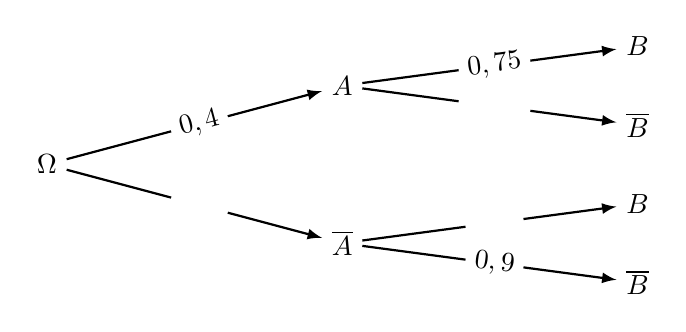
\begin{tikzpicture}
	\tikzstyle{fleche}=[->,>=latex,thick]
	\tikzstyle{noeud}=[]\tikzstyle{feuille}=[]
	\tikzstyle{etiquette}=[pos=0.52,sloped,fill=white]
	\def\DistanceInterNiveaux{3}\def\DistanceInterFeuilles{1}
	\def\NiveauA{(0)*\DistanceInterNiveaux}
	\def\NiveauB{(1.25)*\DistanceInterNiveaux}
	\def\NiveauC{(2.5)*\DistanceInterNiveaux}
	\def\InterFeuilles{(-1)*\DistanceInterFeuilles}
	\node[noeud] (R) at ({\NiveauA},{(1.5)*\InterFeuilles}) {$\Omega$};
	\node[noeud] (Ra) at ({\NiveauB},{(0.5)*\InterFeuilles}) {$A$};
	\node[feuille] (Raa) at ({\NiveauC},{(0)*\InterFeuilles}) {$B$};
	\node[feuille] (Rab) at ({\NiveauC},{(1)*\InterFeuilles}) {$\overline{B}$};
	\node[noeud] (Rb) at ({\NiveauB},{(2.5)*\InterFeuilles}) {$\overline{A}$};
	\node[feuille] (Rba) at ({\NiveauC},{(2)*\InterFeuilles}) {$B$};
	\node[feuille] (Rbb) at ({\NiveauC},{(3)*\InterFeuilles}) {$\overline{B}$};
	\draw[fleche] (R)--(Ra) node[etiquette] {$0,4$};
	\draw[fleche] (Ra)--(Raa) node[etiquette] {$0,75$};
	\draw[fleche] (Ra)--(Rab) node[etiquette] {$\phantom{0,25}$};
	\draw[fleche] (R)--(Rb) node[etiquette] {$\phantom{0,6}$};
	\draw[fleche] (Rb)--(Rba) node[etiquette] {$\phantom{0,1}$};
	\draw[fleche] (Rb)--(Rbb) node[etiquette] {$0,9$};
\end{tikzpicture}

\begin{enumerate}
	\item Compléter l'arbre.
	\item Déterminer les valeurs de $P(A)$ et $P_{\overline{A}}(B)$.
	\item 
	\begin{enumerate}
		\item Calculer $P(A \cap B)$ et $P\big(\overline{A} \cap B\big)$.
		\item En déduire la valeur de $P(B)$.
	\end{enumerate}
\end{enumerate}
\end{minipage}
\hfill
\begin{minipage}{0.49\linewidth}
\papierseyes*{11}{10}
\end{minipage}

\end{document}

\papierseyes{20}{2}